
\section{Locating like-species using vector clustering}
In reducing the various representation for each species to two-dimension, we may represent them as two-dimensional plots. For a small number of samples, we can then visually apply our pattern recognition abilities to group nearby species and explore any structural similarities through interaction. Since this is often a time consuming and taxing process, we may employ the use of various vector clustering methods\footnote{Vector clustering is the grouping of data based on their proximity or density to other nearby points}.  Each of these methods can produce

\begin{figure}[H]
     \centering

         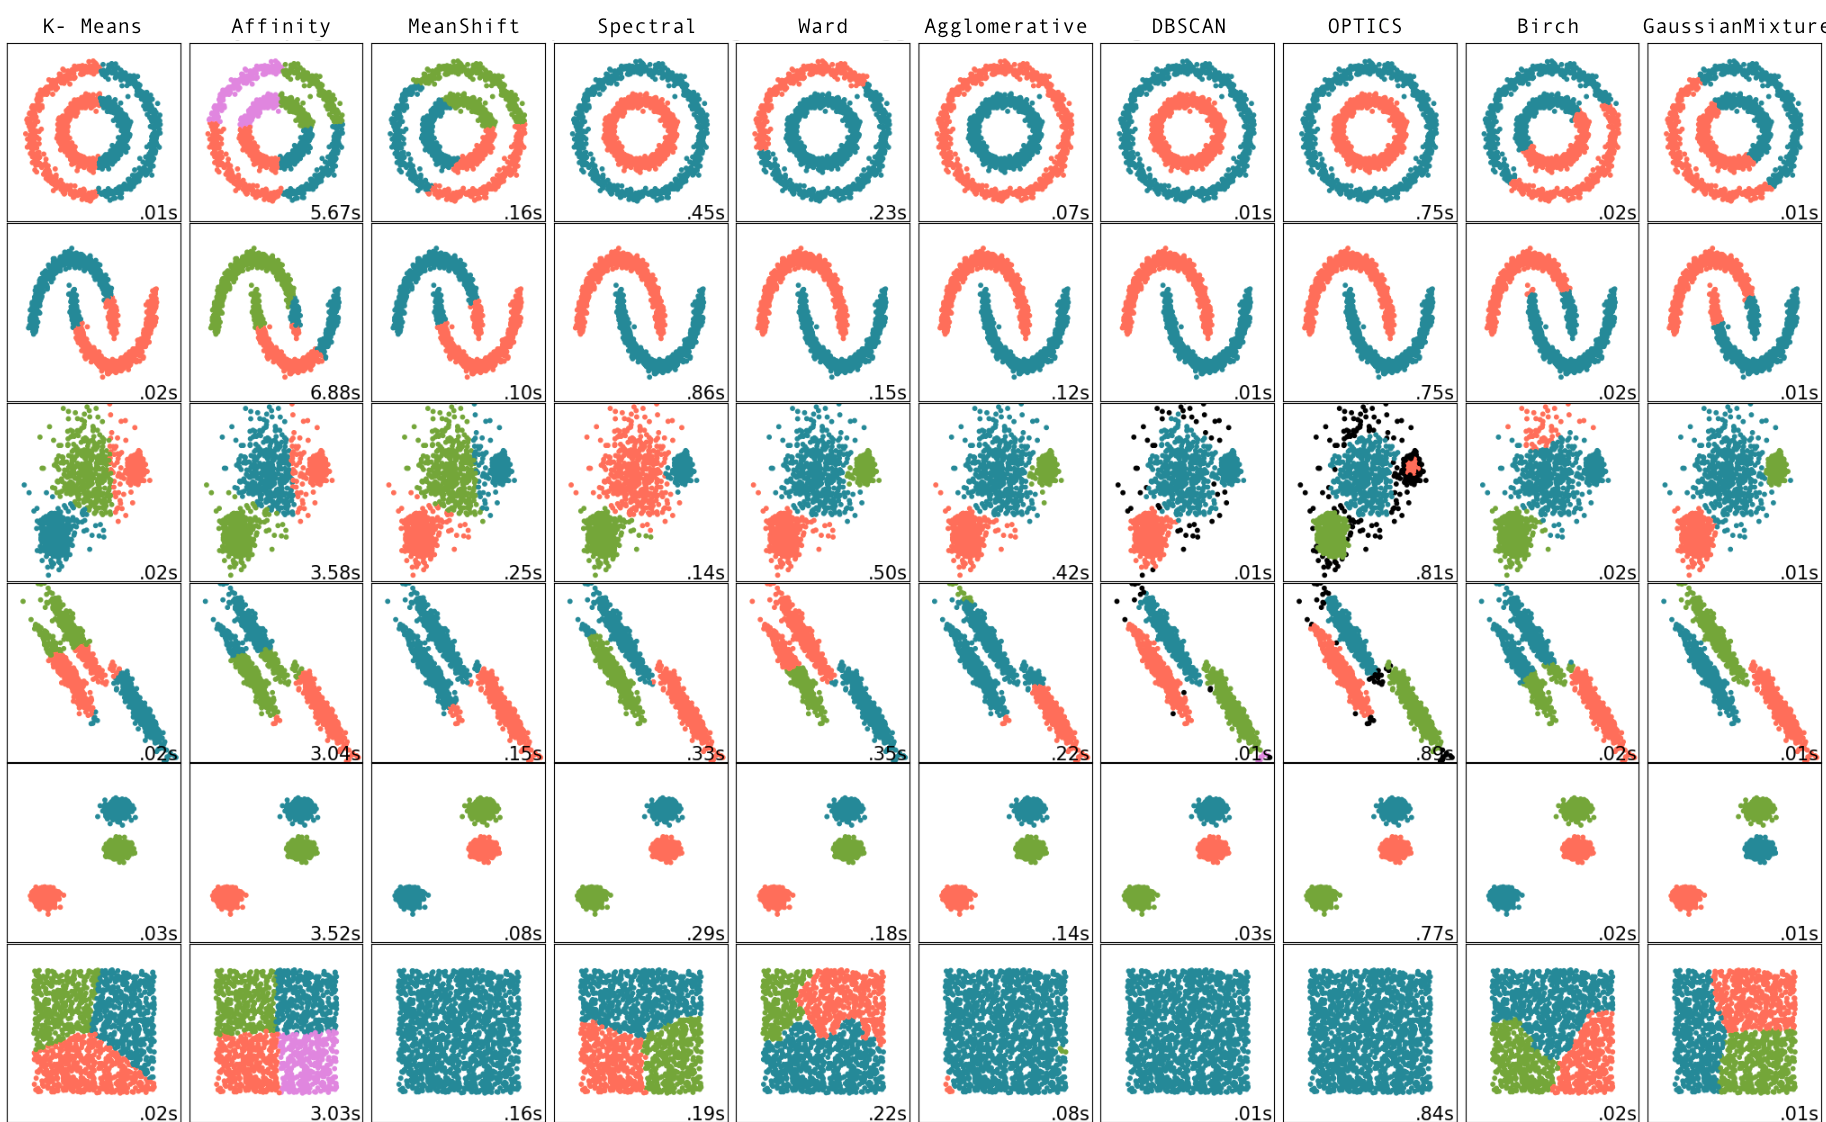
\includegraphics[width=\textwidth]{4fig/clustereval.png}

        \caption{A comparison of different clustering methods on a toy dataset. Source: \cite{clustereval}}
        \label{fig:clustereval}
\end{figure}

\subsection{Clustering Methods}


We run models and reduce to 2D space. This allows for the use of the vector clustering algorithms described in Section XX. To access how well this perfom on the dimensionally reduced dataset we can rely on the silhouette coefficient.

\subsection{Cluster Evaluation}


\subsection{Clustering (Silhouette) coefficient}
The silhouette measure is a tool used for acessing the validity of a set of clusters. Here each cluster is represented as a silhouette, based on the comparison of its tightness and separation. To calculate the silhoette coefficient we look at the intra-cluster $a$ and the mean inter-cluster\footnote{Inside and between different clusters.} distance $b$. The silhouette cluster can then be described using \ref{silhouette,sklearn}:

\begin{equation}
s(i) = \frac{b(i)-a(i)}{\max{ a(i), b(i)}}
\end{equation}

This gives a value $-1 \le s(i) \le 1$. Values near zero suggest overlapping clusters, 1 - dense, well-separated clusters and negative values indicate that a sample may have been incorrectly classified. In using this method we can get an overview of how well individual objects lie within their assigned cluster.

\subsection{Feature Extraction}
Once we have established how well the highlighted clusters reflect the data we then have to determine which features they best represent. The main problem that arises with this is the convolution of many different features into one cluster within the feature space. In separating these ...

Random Forrest Classifier from sklearn, top n features.
https://github.com/MaartenGr/CustomerSegmentation/blob/master/Customer%20Segmentation.ipynb
https://www.ncbi.nlm.nih.gov/pmc/articles/PMC5732374/

The only downside is that Random Forrests are in themselves ML techniques which also need to be evaluated. To do this, as they are simply being used as indicators of cluster properties which we are to explore further, we can initiate a collection of $n$\footnote{In this case 10?} random Forrest classifiers










\subsection{Visualisation and Clustering}

%
% \subsubsection{Graph visualisation}
% In order to represent graphs we take an approach similar to previous chapters. Here nodes are represented as circles, sized according to the number of functional groups or the amount a specific group exists. In order to reduce clutter links between spatially distant species are bundled (\cite{edgebundle}), whilst those close together are not changed (a technique similar to that used in \cite{graphtsne}. Nodes are assigned properties, and may be matched using full or partial matches to their names, functional groups or smiles strings. Interactivity through the use of mouseover events  are used to accomplish the level of exploratory data analysis required for this task.

\subsubsection{Reduced Dimension space}
Data provided will be reduced into two dimensions. Although this may not be the best method for preserving its information, it allows us to visually access what information is retained when we heavily compress our inputs.

To evaluate this we shall represent it in an adapted x-y scatter plot. The simplest way to achieve this is by normalizing the algorithm output between the numbers of {0,1}.


\subsubsection{Automated selection of clusters}
There exist many methods of vector clustering. Methods, such as k-means[REF], although fast and simple to understand, cannot capture the splits between nonlinear representations of data. Additionally, they require the number of clusters to be supplied, at which point, it is usually easier to manually `brush' the nodes in question on an interactive plot.

Density-based clustering methods such as GMM and DBSCAN \cite{scikit,DBSCAN} tend to be preferable. For instance, DBSCAN looks at the distribution of data residing a defined (eps?) distance around a point. This is useful as the number of clusters present does not need to be pre-defined. The method that shall be used (OPTICS [ref])\footnote{ If using Python 2, the library for this needs to be extracted from the scikit-learn library for python 3 package and altered to run with the previous version. (See copy in attached code.)}. This is an adaptation of the DBSCAN algorithm that works... and does not require the specification of a minimum distance between points. Instead, we specify a gradient for the distribution and the minimum number of points for a cluster to be classified.

Cluster will be evaluated using the methods discussed in section [see above], and run under a range of conditions before picking the best combination.

\paragraph{Four Colours Theorem}
When plotted, the number of clusters detected often exceeds the number of categorical colours available. In an attempt to reduce these we apply a greedy implementation of the four colours theorem \cite{fourcolour}.
The four colour theorem states that each map may be coloured with no more than 4 colours. More explicitly that any two regions (e.g. a country if we are looking at world map may not share the same colour as this causes ambiguity between results. This is especially true when trying to visually differentiate different clusters by colour. The algorithm developed uses the Delaunay tesselation scripts contained within DataDrivenDocuments.js (d3js) \cite{d3js}. This partitions our plane into polygon-regions with boundaries at the furthest distance from each point (Voronoi cells) \cite{delaunay}. Using this we may start at a randomly assigned cell providing it with a colour. We then recursively iterate through all neighbours assigning them with the lowest possible colour that does not occur within any of their neighbours. Although such a greedy approach does not produce an optimum result it allows for the colouring of data with $\le 5$ distinct colours.


\qfig{4fig/4colour.png}{fig:4col}{An example 4 colour matching using the first implementation of the above algorithm - Observable Notebook : \cite{4colobs}}{.7\textwidth}

\paragraph{Exposing data}
Since much of the initial exploration was done using manual intervention and interaction, we found clusters of nodes would often occupy the same space within a graph. There exist two solutions, one of which involves reducing the size of the dots to prevent overlaps, however, this does not always prove useful, and often results in difficulties when trying to select a node. The alternative is to apply the d3 force-directed algorithm combined with a level of collision detection. \\

Nodes are configured in such a way that experience a strong attraction force to their respective $(x,y)$ coordinates. The collision algorithm then repels them from existing within the radius of other nodes. This transforms any clusters of stacked nodes into adjacent groupings around the common centre, in turn making it possible to select each node individually.

\paragraph{Gooey Effect (Gaussian Blur)}
When comparing the existence of certain properties it is often to use colour as an encoding. To prevent distraction through the recognition of separate points, it may be found that blurring adjacent points into a single mass whilst representing information of interest using a variable colour gradient, reduces the cognitive load on the end-user (especially when it comes to dense plots consisting of multiple points.

The simplest way to do this is to apply a gooey-style filter (a method used for creating water droplet style effects in web animations). This works through the merging of ... and a Gaussian blurring matrix of INSERT HERE.
